\documentclass[letterpaper,onecolumn,openany,nodeprecatedcode]{dndbook}

% Use babel or polyglossia to automatically redefine macros for terms
% Armor Class, Level, etc...
% Default output is in English; captions are located in lib/dndstring-captions.sty.
% If no captions exist for a language, English will be used.
%1. To load a language with babel:
%	\usepackage[<lang>]{babel}
%2. To load a language with polyglossia:
%	\usepackage{polyglossia}
%	\setdefaultlanguage{<lang>}
\usepackage[english]{babel}
%\usepackage[italian]{babel}
% For further options (multilanguage documents, hypenations, language environments...)
% please refer to babel/polyglossia's documentation.

\usepackage[utf8]{inputenc}
\usepackage[singlelinecheck=false]{caption}
\usepackage{lipsum}
\usepackage{listings}
\usepackage{shortvrb}
\usepackage{stfloats}
\usepackage{graphicx}
\usepackage{wrapfig}

\captionsetup[table]{labelformat=empty,font={sf,bf,},skip=0pt}

\MakeShortVerb{|}

\lstset{%
  basicstyle=\ttfamily,
  language=[LaTeX]{TeX},
  breaklines=true,
}


\begin{document}

\begin{wrapfigure}{r}{0.2\textwidth}
    \begin{center}
        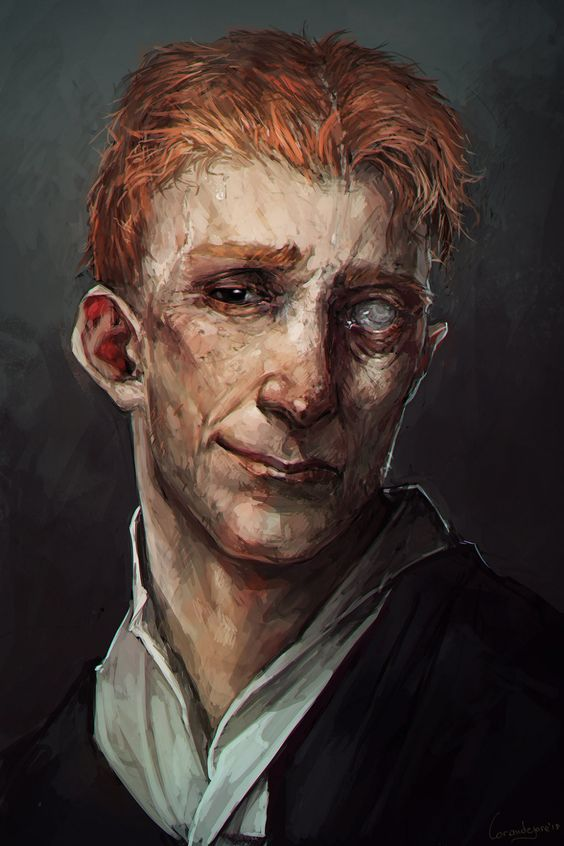
\includegraphics[width=0.2\textwidth]{img/harold}
    \end{center}
\end{wrapfigure}

\section{Adepti dobrodružení}
\section {Harold ‘Jizva’ z Kremle}
\subsubsection{Bojovník s obouručními těžkými zbraněmi}
Na to že je lyrista má neobvykle vypracovanou postavu a silné ruce, div že ten drobný nástroj v rukou omylem nerozdrtí. Zjevně se vyzná ve městě i divočině a těžká práce mu není cizí. Ošklivá jizva na obličeji mu dává spíš zastrašující výraz kriminálního živla než potulného barda i když hadry by na to měl.
\vspace{15 mm}

\begin{wrapfigure}{r}{0.2\textwidth}
    \begin{center}
        
\includegraphics[width=0.2\textwidth]{img/yasmina.jpg} 
    \end{center}
\end{wrapfigure}
\section{Yasmina}
\subsubsection{Kouzelnice školy věštění}
Nadšená lidská kouzelnice, toužící po dobrodružství, která stále nosí na čele diadém. Tvrdí, že nucené práce dělala, protože odmítla mocného úchylného šlechtice a její pravník to pokazil a z ní jako oběti se ještě stal viník. Zdá se být velmi chytrá, ošklivá taky není, pohybuje se s lehkostí kočky, ale nic těžšího než koště jí do ruky určitě nikdy nedali. Vyzná se v historii a magii. Při nucených pracích prý někoho zachránila před úrazem, díky své věštecké vizi, ale přesto mi na ní něco nesedí.

\vspace{15 mm}

\begin{wrapfigure}{r}{0.2\textwidth}
    \begin{center}
        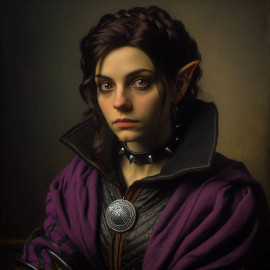
\includegraphics[width=0.2\textwidth]{img/silgrid.jpg} 
    \end{center}
\end{wrapfigure}

\section{Silgrid Uhlocopá}
\subsubsection{Trpasličí neřád}
Důvěřivá, zbožná trpaslice s tmavým kovovým obojkem. Číší z ní soucit a pochopení, ale asi bude trochu blázen, mám pocit, že cizí pocity příliš prožívá. Oproti jiným trpaslíkům je spíš drobnější a hubenější a v dolech by asi dlouho nevydržela. Pohybuje se však rychle a má dobrou mušku. Často se nenápadně k něčemu modlí v temných uličkách, když se zrovna nikdo nedívá. Pořád nosí černý hardy a přes všechny ty její divný zvyky se s ní docela dobře povídá.

\vspace{20 mm}

\begin{wrapfigure}{r}{0.2\textwidth}
    \begin{center}
        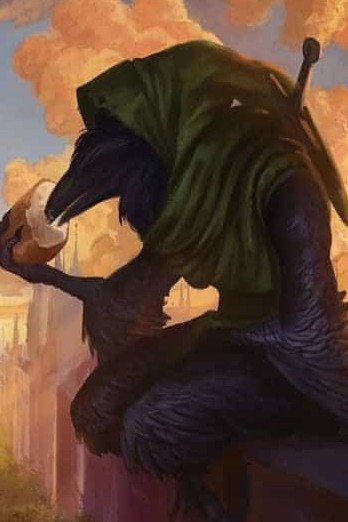
\includegraphics[width=0.2\textwidth]{img/sally.jpg} 
    \end{center}
\end{wrapfigure}

\section{Sally “Kavka” Horst}
\subsection{Kenku hraničář druidský bojový styl}
Tajnůstkářský šedočerný Kenku o kterém kolují zvěsti, že kdysi patřil k městské hlídce. Nedokáže mluvit, jen napodobuje ostatní hlasy a zvuky. Není moc silný což u ptačí rasy není tak divný. Vypadá že koná s rozvahou a nenechá se příliš unášet emocemi. Chodí klidně a opatrně vnímá okolí a při každém šustnutí je napozoru. Přírodě, zdá se rozumí a ve městě se nenechá ničím zaskočit. Působí čestně, ale co dělá tady a proč ho vyhodili z městské hlídky, nikomu neřekl.


\end{document}
